\documentclass[a4paper, 12pt, titlepage, fleqn]{article}

%Taal: Nederlands ("Inhoudsopgave", "Hoofdstuk",...)
\usepackage{graphicx}
\usepackage{subcaption}
\usepackage{amsmath, amssymb, textcomp, mathtools}
\usepackage{geometry}
	\geometry{a4paper, left=20mm, right=20mm, top=20mm, bottom=20mm}
\setlength{\mathindent}{1cm}
%Hyperlinks
\usepackage{hyperref}
\usepackage{subcaption}

%Opmaak hyperlinks
\hypersetup{colorlinks=false,	urlcolor=cyan,pdfborder=0 0 0}
\usepackage[framed,numbered,autolinebreaks,useliterate]{mcode}
%geen indents
\setlength\parindent{0pt}
\usepackage{listings}
\lstset{
language=Matlab, % choose the language of the code
%basicstyle=10pt, % the size of the fonts that are used for the code
numbers=left, % where to put the line-numbers
numberstyle=\footnotesize, % the size of the fonts that are used for the line-numbers
stepnumber=1, % the step between two line-numbers. If it's 1 each line will be numbered
numbersep=5pt, % how far the line-numbers are from the code
%backgroundcolor=\color{grey}, % choose the background color. You must add \usepackage{color}
showspaces=false, % show spaces adding particular underscores
showstringspaces=false, % underline spaces within strings
showtabs=false, % show tabs within strings adding particular underscores
frame=single, % adds a frame around the code
%tabsize=2, % sets default tabsize to 2 spaces
captionpos=b, % sets the caption-position to bottom
breaklines=true, % sets automatic line breaking
breakatwhitespace=false, % sets if automatic breaks should only happen at whitespace
escapeinside={\%*}{*)} % if you want to add a comment within your code
}


\usepackage[dutch]{babel}
\begin{document}

\title{\textbf{Numerieke Modellering en Benadering: Chebyshev veeltermen}}
\author{Sander Prenen}

\date{15 april 2020}
\begin{titlepage}
	\maketitle
	\thispagestyle{empty}
\end{titlepage}

\newpage
\tableofcontents
\newpage
\section{Inleiding}
In dit practicum worden de benaderingseigenschappen van Chebyshev veeltermen van de eerste soort. Deze veeltermen blijken uiterst geschikt voor het benaderen van eindige, re\"ele functies met behulp van de continue kleinste kwadratenbenadering. Ook zijn hun nulpunten vaak een uitstekende keuze voor de abscissa voor veelterminterpolatie. In sectie \ref{sec:benadering} wordt dieper ingegaan op de benaderingseigenschappen, terwijl in sectie \ref{sec:interpolatie} de interpolatie besporken wordt.

\section{Continue kleinste kwadratenbenadering met Chebyshev veeltermen}
\label{sec:benadering}
In deze sectie wordt geprobeerd continue functies op eindige, re\"ele intervallen te benaderen aan de hand van Chebyshev-veeltermen van de eerste soort. Dit zijn veeltermen die voldoen aan de volgende voorwaarde: $T_k(x) = \cos(k \arccos (x))$ voor $x \in [-1,1]$ en $k = 0,1,2,\ldots$ De veeltermen vormen een basis voor de ruimte $V_n$, een deelvectorruimte van $C([-1,1])$. 


\subsection{Beste benadering in $V_n$}
Indien de basisvectoren $T_k(x)$ orthogonale vectoren zijn, geldt volgende uitdrukking voor de beste benadering $y_n(x)$ voor een functie $f(x) \in C([-1,1])$:
\begin{equation}
y_n(x) = \sum_{k=0}^na_kT_k(x) \hspace{1cm} \text{met} \hspace{1cm} a_k = \frac{(f,T_k)}{(T_k,T_k)}
\label{eq:beste_benadering}
\end{equation}

Met als scalair product:
\begin{equation*}
(f,g) = \int_{-1}^1\frac{f(x)g(x)}{\sqrt{1-x^2}}dx
\end{equation*}

Om deze formule te kunnen gebruiken, moet dus worden aangetoond dat de basisvectoren orthogonaal zijn. Dit wil zeggen dat alle onderlinge scalaire producten nul zijn, tenzij dat van een basisvector met zichzelf. 

\subsubsection{Orthogonaliteit van de basisvectoren $T_k$}
\label{subsec:scalaireProducten}
In deze sectie wordt de orthogonaliteit van de basisvectoren bekeken. Hiervoor moeten alle onderlinge scalaire producten bepaald worden. Dit wordt gedaan in drie gevallen:
\begin{itemize}
\item $k = l = 0$:
\begin{equation*}
(T_k,T_l) = \int_{-1}^1 \frac{T_0^2(x)}{\sqrt{1-x^2}}dx = \int_{-1}^1 \frac{1}{\sqrt{1-x^2}}dx =\left[\arcsin(x)\right]_{-1}^1 = \pi
\end{equation*}
\item $k = l \neq 0$:
\begin{equation*}
(T_k,T_l) = \int_{-1}^1\frac{T_k^2(x)}{\sqrt{1-x^2}}dx = \int_{-1}^1\frac{\cos^2(k \arccos(x))}{\sqrt{1-x^2}}dx = \frac{2\pi k + \sin(2\pi k)}{4k} = \frac{\pi}{2}
\end{equation*}
\item $k \neq l$:
\begin{align*}
(T_k,T_l) &= \int_{-1}^1\frac{T_k(x)T_l(x)}{\sqrt{1-x^2}}dx = \int_{-1}^1\frac{\cos(k \arccos(x))\cos(l \arccos(x))}{\sqrt{1-x^2}}dx\\
&=\frac{1}{2}\int_{-1}^1\frac{\cos((k-l)\arccos(x))}{\sqrt{1-x^2}}dx + \frac{1}{2}\int_{-1}^1\frac{\cos((k+l)\arccos(x))}{\sqrt{1-x^2}}dx\\
&=\frac{1}{2}\frac{\sin((k-l)\pi)}{k-l} + \frac{1}{2}\frac{\sin((k+l)\pi)}{k+l} = 0
\end{align*}
\end{itemize}
Alle scalaire producten zijn nul, behalve die van basisvectoren met zichzelf. De vectoren zijn dus orthogonaal.

\subsubsection{Beste benadering}
Doordat de basisvectoren orthogonaal zijn, kan formule (\ref{eq:beste_benadering}) gebruikt worden. In deze sectie worden de co\"effic\"enten $a_k$ bepaald.
\begin{align*}
a_k &= \frac{(f,T_k)}{(T_k,T_k)} = \frac{1}{(T_k,T_k)}\int_{-1}^1\frac{f(x)T_k(x)}{\sqrt{1-x^2}}dx = \frac{1}{(T_k,T_k)}\int_{-1}^1\frac{f(x)\cos(k \arccos(x))}{\sqrt{1-x^2}}dx\\
&= \frac{1}{(T_k,T_k)}\int_\pi^0\frac{f(\cos \theta)\cos(k\theta)(-\sin(\theta))}{\sqrt{1-\cos^2(\theta)}}d\theta = \frac{1}{(T_k,T_k)}\int_0^\pi f(\cos \theta) cos(k\theta)d\theta
\end{align*}
Dit geeft dus volgende uitdrukking voor $a_k$ gebruikmakend van de uitdrukkingen in sectie \ref{subsec:scalaireProducten}:
\begin{align}
a_k = \begin{cases}
\frac{1}{\pi}\int_0^\pi f(\cos \theta)d\theta, & k = 0\\
\frac{2}{\pi}\int_0^\pi f(\cos \theta)\cos(k\theta)d\theta, & k > 0
\end{cases}
\label{eq:a_K}
\end{align}



\subsection{Evalueren van de Chebyshev veeltermen}
Om de beste benadering numeriek te bepalen, moet vergelijking (\ref{eq:beste_benadering}) ge\"evalueerd worden. De functie \texttt{evalCheb} geeft een vector $v = (f_1, f_2, \ldots, f_N) \in \mathbb{R}^N$ terug. Deze vector wordt bekomen uit inputvectoren $a = (a_0,a_1,\ldots, a_n) \in \mathbb{R}^{n+1}$ en $x = (x_1,x_2,\ldots,x_N) \in \mathbb{R}^N$ op de volgende manier:
\begin{equation*}
f_i = y_n(x_i) = a_0T_0(x_i) + a_1T_1(x_i) + \ldots + a_nT_n(x_i)
\end{equation*}

In Listing \ref{lst:evalCheb} wordt de MATLAB code voor deze berekening weergegeven.

\lstinputlisting[caption={evalCheb.m}, label = {lst:evalCheb}]{../evalCheb.m}


\subsection{Bepalen van de co\"effici\"enten}
Voor het bepalen van de co\"effici\"enten $a_k$ kan vergelijking (\ref{eq:a_K}) gebruikt worden. Deze vergelijking kan met behulp van de trapeziumregel voor numerieke integratie met een discretizatie bestaande uit $n$ intervallen, benaderd worden door:
\begin{align*}
a_k \approx \frac{1}{n}f(1) + \frac{2}{n}\sum_{l=1}^{n-1}f\left(\cos\left(\frac{l\pi}{n}\right)\right)\cos\left(k\frac{l\pi}{n}\right) + \frac{(-1)^k}{n}f(-1), \hspace{1cm} 0 < k \leq n
\end{align*}
Hieruit volgt dat de co\"effici\"enten $a_k$ kunnen berekend worden als de DCT van de rij:
\begin{align}
f(z_{0,n}),f(z_{1,n}), \ldots, f(z_{n,n})
\label{eq:DCTrij}
\end{align} 
Hierin is $z_{l,n} = cos(l\pi/n)$. Deze punten zijn de extrema van $T_k(x)$ aangezien dit de nulpunten zijn van de eerste afgeleide van $T_k(x)$.

\begin{align*}
\frac{dT_k(x)}{dx} &= \frac{d}{dx}\cos(k\arccos(x)) = -\sin(k \arccos(x))\cdot k \cdot - \frac{1}{\sqrt{1-x^2}}
\end{align*}

De afgeleide wordt nul als $k=0$ of $\sin(k \arccos(x)) = 0$. In het tweede geval herleidt dit zich tot:
\begin{align*}
k\arccos(x) = l\pi \Leftrightarrow x = \cos\left(\frac{l\pi}{k}\right)
\end{align*}

In de functie \texttt{approxCheby} wordt de DCT van de rij in vergelijking (\ref{eq:DCTrij}) bepaald. De code van deze functie kan gevonden worden in Listing \ref{lst:approxCheby} weergegeven.

\lstinputlisting[caption={approxCheby.m}, label = {lst:approxCheby}]{../approxCheby.m}


\subsection{Benaderen van een functie}
De algoritmes die in Listing \ref{lst:evalCheb} en \ref{lst:approxCheby} te zien zijn, kunnen gebruikt worden bij het benaderen van een willekeurige functie in $C([-1,1])$. Om een functie te benaderen worden de co\"effic\"enten $a_k$ bepaald met \texttt{approxCheby}. Deze co\"effic\"enten worden meegegeven aan \texttt{evalCheb}. De punten waarin de benadering ge\"evalueerd moet worden meegegeven in de $x$ vector. In dit geval wordt gekozen voor 200 equidistante punten tussen $-1$ en $1$.

In figuur \ref{fig:rungeFunctie} worden de beste benaderingen voor de Runge functie in ruimtes $V_2$ tot $V_{20}$ weergegeven. De Runge functie heeft als voorschrift $f(x) = \frac{1}{25x^2+1}$. Figuur \ref{fig:rungeFout} toont de maximale afwijking $d(y_n,f) = \max_{x \in [-1,1]}|y_n(x)-f(x)|$, in functie van de graad van de benaderende veelterm. 
\begin{figure}
\centering
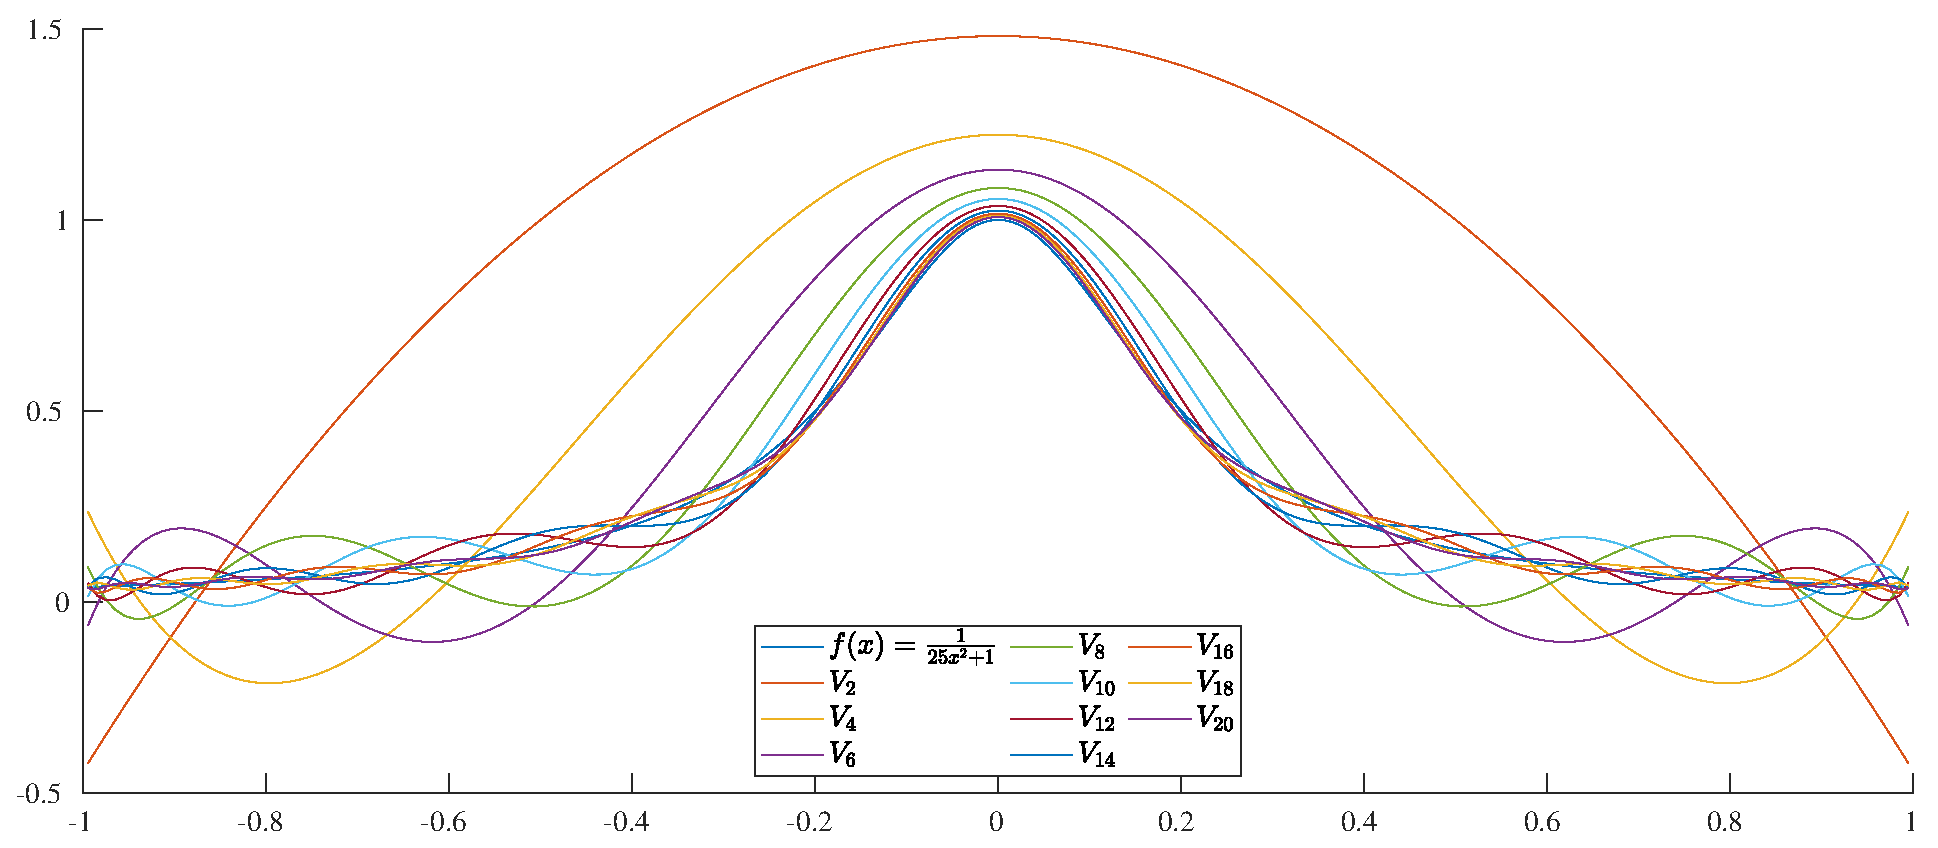
\includegraphics[scale=0.5]{../Afbeeldingen/rungeBenadering.eps}
\caption{De beste benaderingen van de Runge functie in de ruimtes $V_2$ tot $V_{20}$.
\label{fig:rungeFunctie}}
\end{figure}

\begin{figure}
\centering
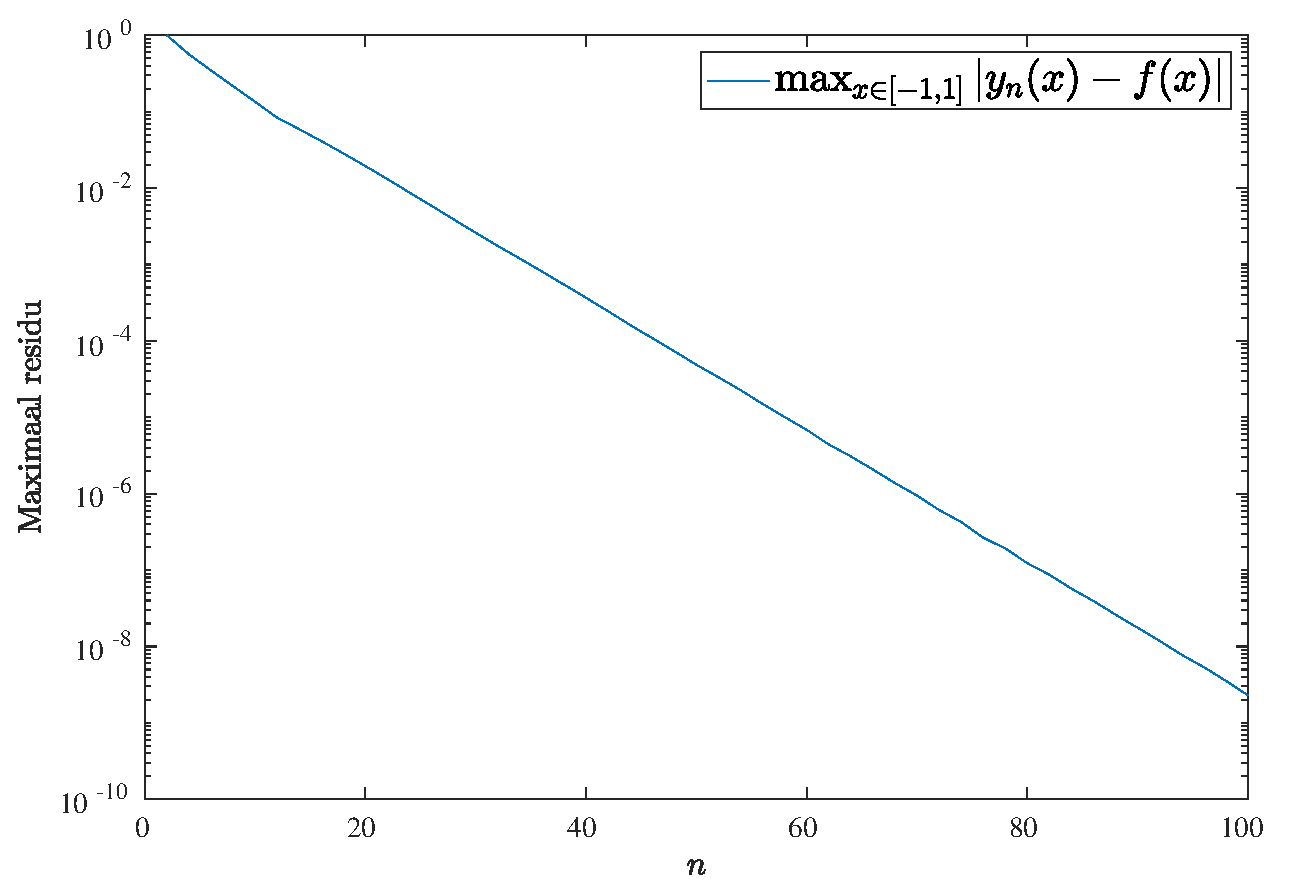
\includegraphics[scale=0.5]{../Afbeeldingen/rungeFout.eps}
\caption{De maximale fout voor de benadering van de runge functie in de ruimtes $V_2$ tot $V_{100}$.
\label{fig:rungeFout}}
\end{figure}

\section{Interpolatie in Chebyshev knooppunten}
\label{sec:interpolatie}
Veeltermen van graad $n-1$ kunnen een functie interpoleren in $n$ interpolatiepunten. De interpolatiepunten $x_k$, voor $k = 1,2,\ldots,n$, kunnen vrij gekozen worden. Er wordt gezocht naar een veelterm $g(x)$ van graad $n-1$ die de functie $f(x)$ interpoleert zodanig dat de volgende voorwaarde voldaan is:
\begin{align*}
g(x_i) = f(x_i), \hspace{1cm} i = 1,\ldots,n
\end{align*}
De veelterm $g(x)$ kan worden voorgesteld in de vorm $g(x) = \sum_{k=0}^{n-1}c_k\psi_k(x)$. Hierin zijn $\psi_k(x)$ de basisfuncties, in dit geval dus $T_k(x)$. De interpolatievoorwaarden leiden tot volgend lineair stelsel:
\begin{align*}
Mc = B
\end{align*}
De oplossing van dit stelsel zijn de co\"effici\"enten $c_k$. De elementen $M_{ij}$ van de matrix $M$ op rij $i$ en kolom $j$ worden gegeven door:
\begin{align*}
M_{ij} = \psi_j(x_i)
\end{align*}
en de elementen $B_i$ van de vector $B$ worden gegeven door:
\begin{align*}
B_i = f(x_i).
\end{align*}

In de functie \texttt{interpolate} worden de co\"effici\"enten $c_k$ en het conditiegetal van de matrix $M$ berekend. Als invoer verwacht de functie de interpolatiepunten $x_k$ en de te benaderen functie~$f(x)$. De code van deze functie is terug te vinden in Listing \ref{lst:interpolate}.

\lstinputlisting[caption={interpolate.m}, label = {lst:interpolate}]{../interpolate.m}

\subsection{Interpoleren van een functie}
\subsubsection{$\cos(x)$ benaderen}
De functie \texttt{interpolate} wordt gebruikt om de functie $f(x) = \cos(x)$ te benaderen. De co\"effici\"enten $c_k$ worden meegegeven aan de functie \texttt{evalCheb} om de interpolant $g(x)$ te kunnen plotten. Voor de interpolatiepunten $x_k$ worden eerst equidistanten punten gekozen. De resultaten worden voor verschillende $n$-waarden getoond in figuren \ref{lageNCosEqui} en \ref{fig:hogeNCosEqui}. Naarmate $n$ stijgt vertoont de benadering aan de randen meer afwijking ten op zichte van $f(x)$. Bij een te hoge $n$ zoals in figuur \ref{fig:hogeNCosEqui} is de benadering heel slecht doordat de gebruikte methode niet stabiel is bij equidistante interpolatiepunten. Door de interpolatiepunten zo te kiezen dat ze de nulpunten zijn van de $k$-de Chebyshev veelterm, wordt de methode wel stabiel. Deze nulpunten zijn van de vorm:
\begin{align*}
x_i = \cos\left(\frac{\pi(2i-1)}{2k}\right), \hspace{1cm} i = 1,\ldots,k
\end{align*}
In figuren \ref{fig:lageNCosNul} en \ref{fig:hogeNCosNul} zijn de interpolatieveeltermen met deze interpolatiepunten te zien. De fout aan de rand is ook veel kleiner zoals in figuur ... te zien is.


\begin{figure}
\centering
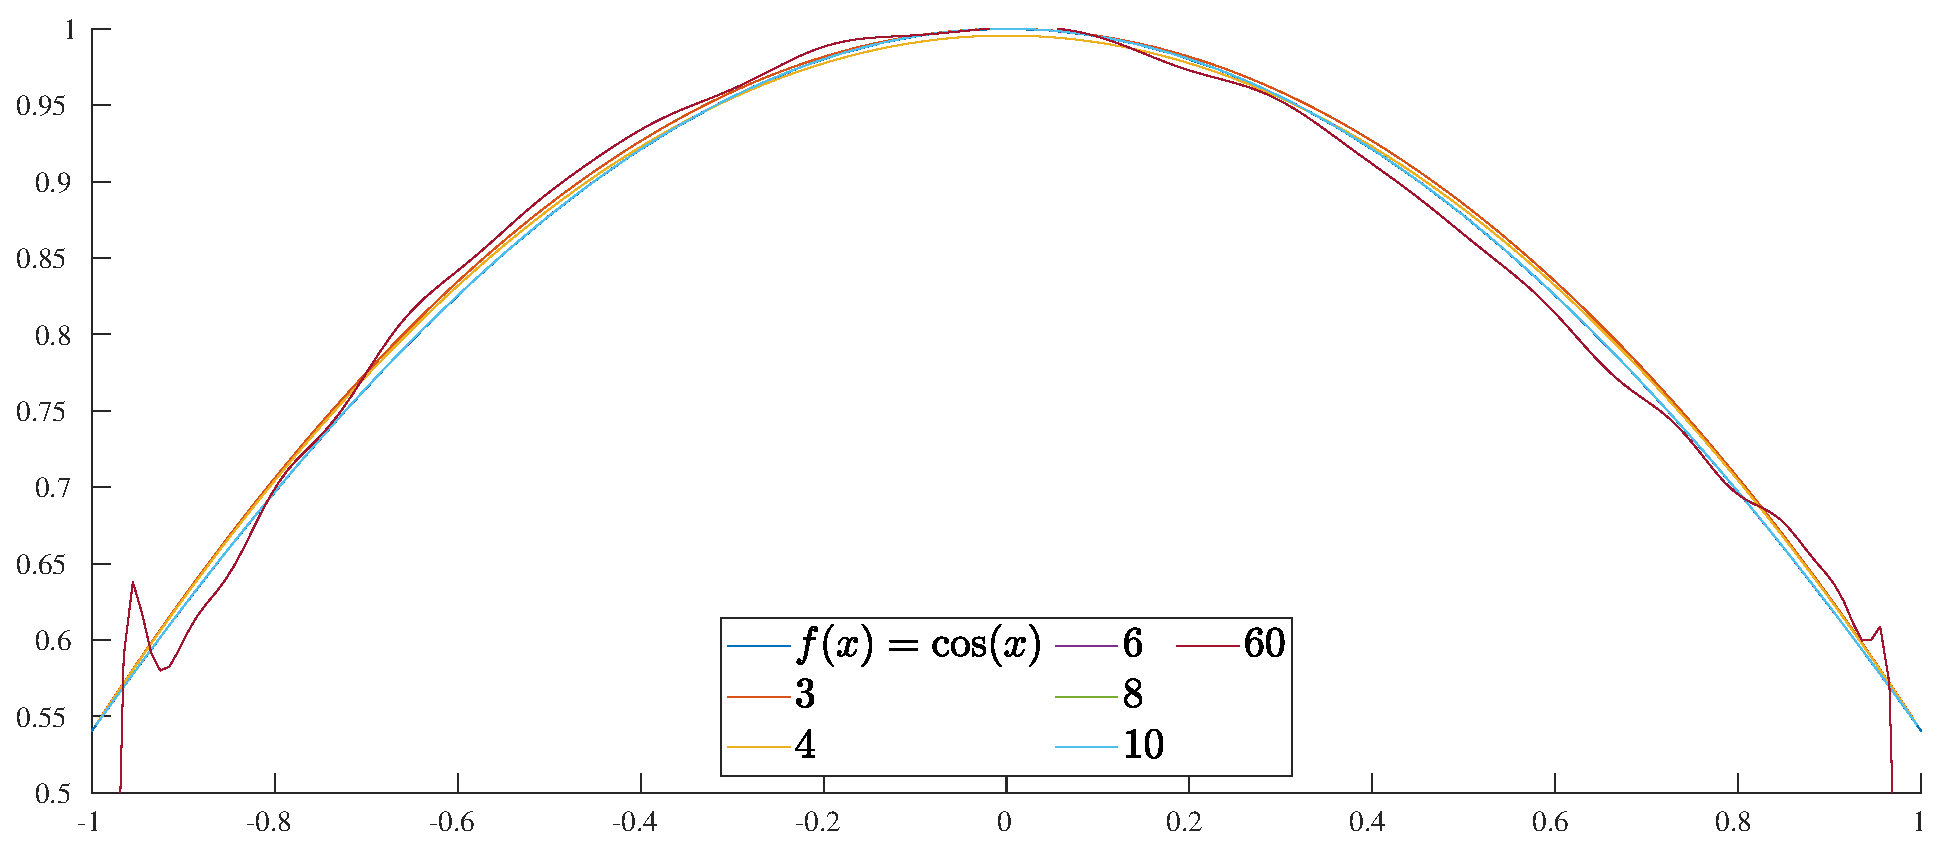
\includegraphics[width=\textwidth]{../Afbeeldingen/cos_equi_laag.eps}
\caption{Benaderingen van de functie $f(x) = \cos(x)$ met een lage $n$ en equidistante interpolatiepunten}
\label{lageNCosEqui}
\end{figure}

\begin{figure}
\centering
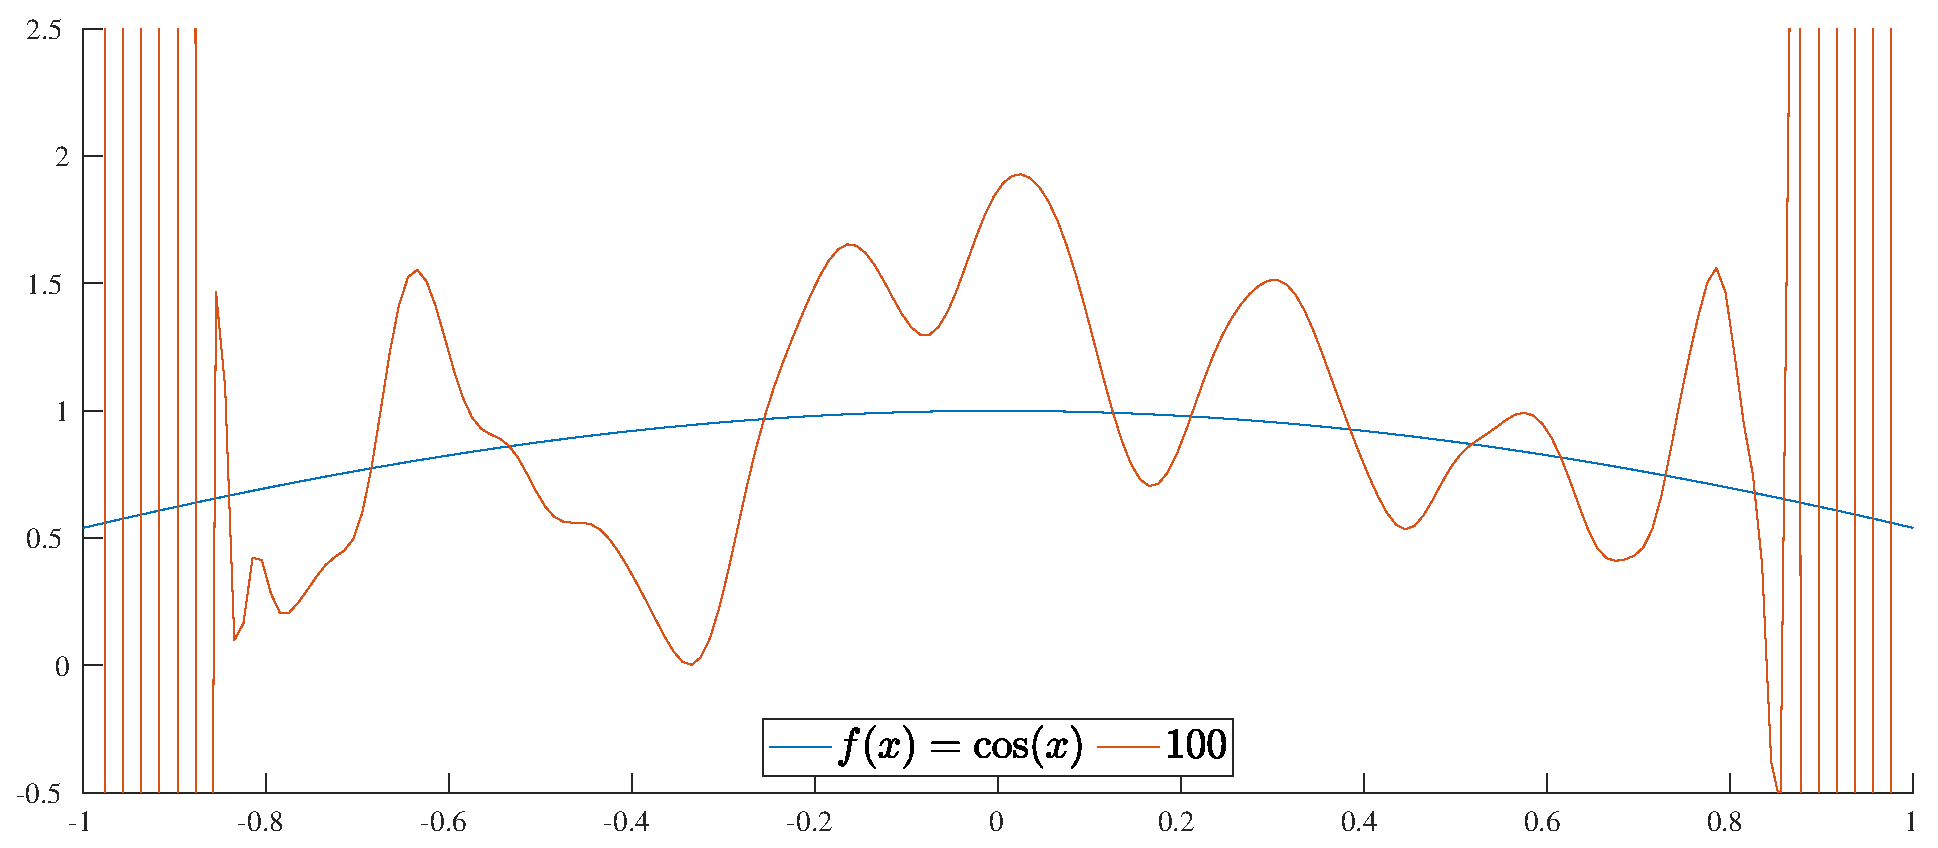
\includegraphics[width=\textwidth]{../Afbeeldingen/cos_equi_hoog.eps}
\caption{Benadering van de functie $f(x) = \cos(x)$ met een hoge $n$ en equidistante interpolatiepunten}
\label{fig:hogeNCosEqui}
\end{figure}

\begin{figure}
\centering
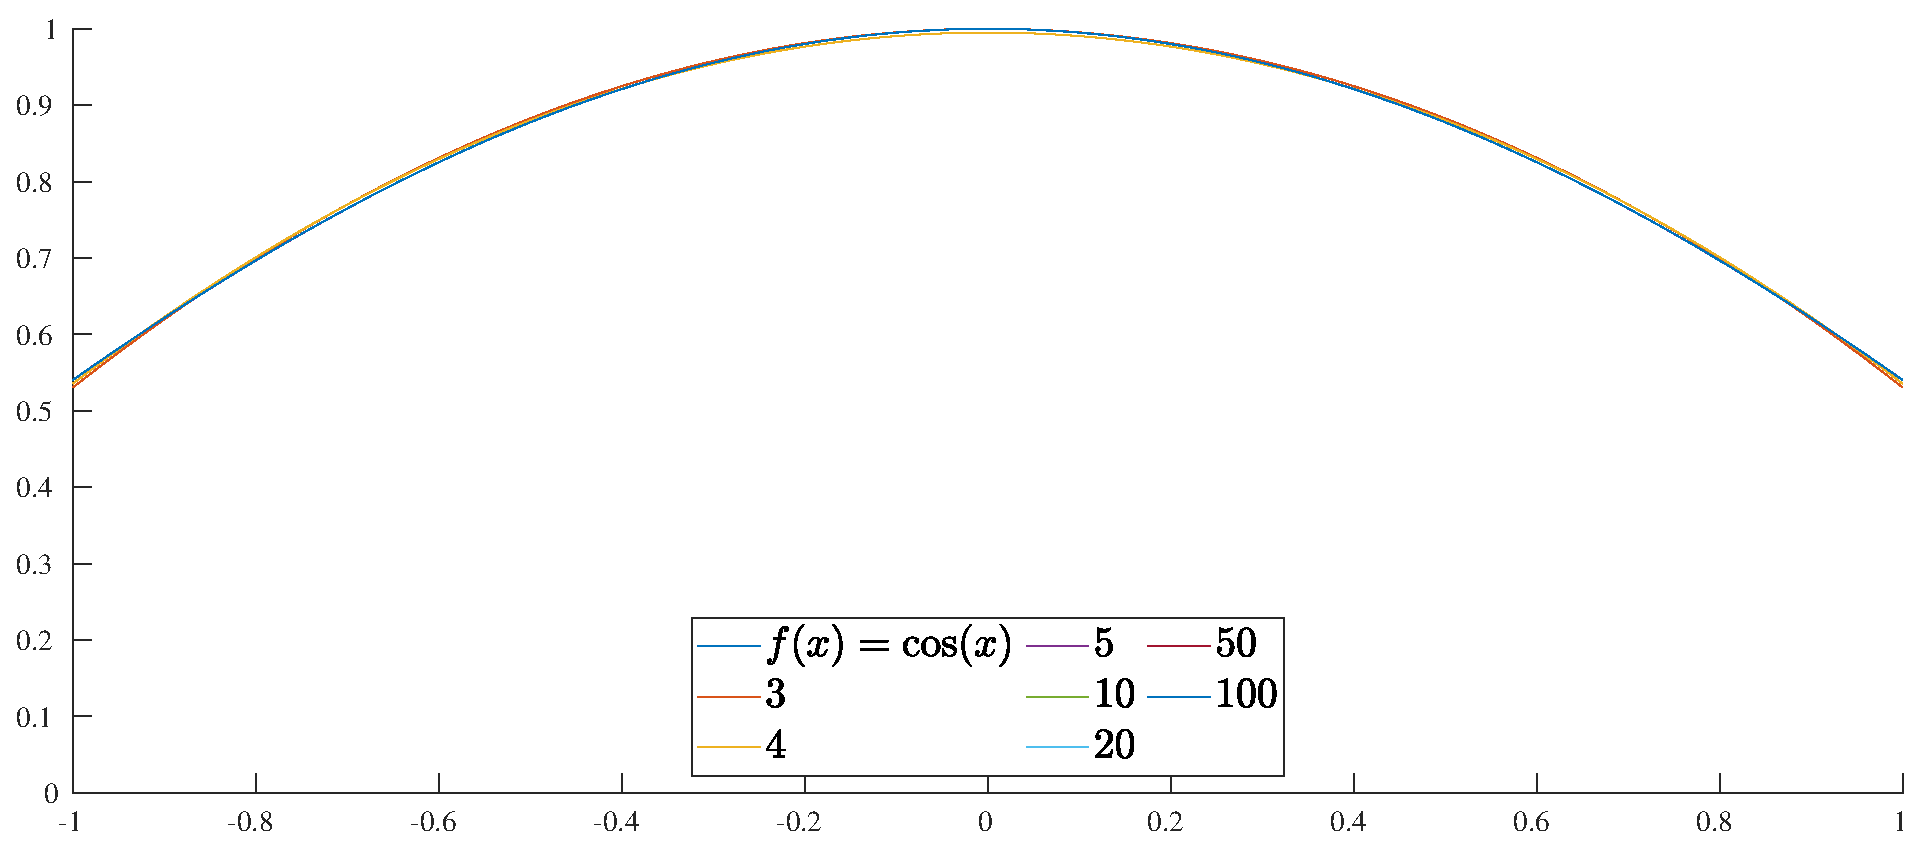
\includegraphics[width=\textwidth]{../Afbeeldingen/cos_nul_laag.eps}
\caption{Benadering van de functie $f(x) = \cos(x)$ met een lage $n$}
\label{fig:lageNCosNul}
\end{figure}

\begin{figure}
\centering
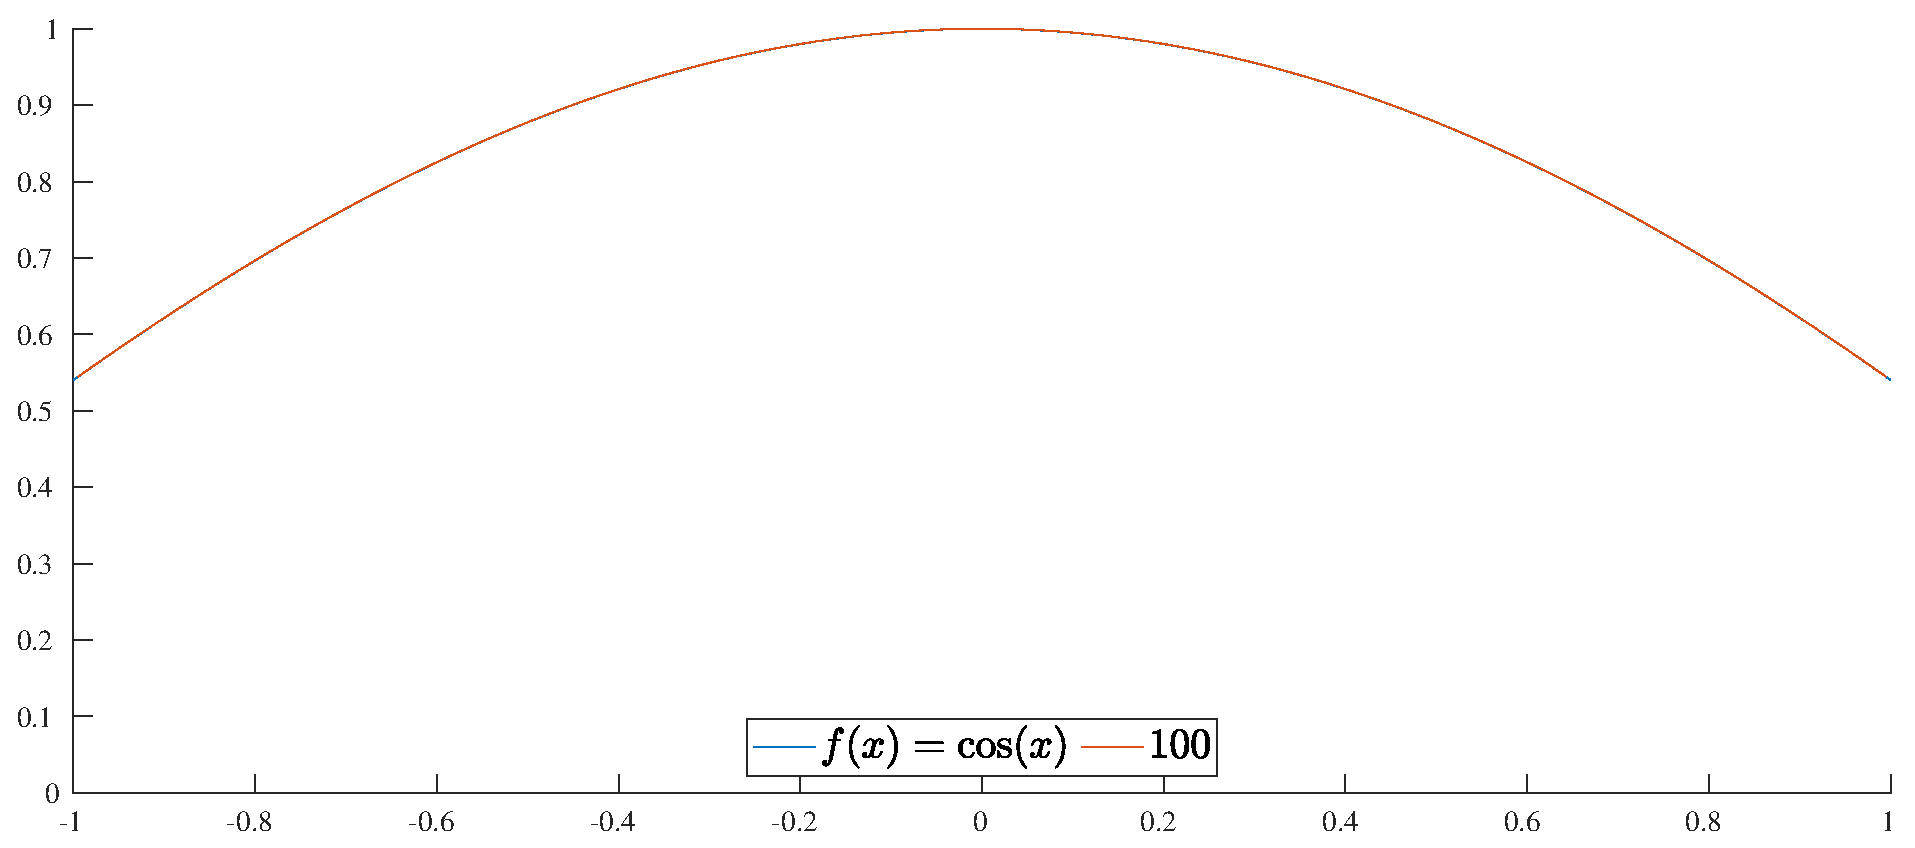
\includegraphics[width=\textwidth]{../Afbeeldingen/cos_nul_hoog.eps}
\caption{Benadering van de functie $f(x) = \cos(x)$ met een hoge $n$}
\label{fig:hogeNCosNul}
\end{figure}

\end{document}